\documentclass[article, onecolumn, 12pt]{IEEEtran}
\IEEEoverridecommandlockouts
% The preceding line is only needed to identify funding in the first footnote. If that is unneeded, please comment it out.
\usepackage{cite}
\usepackage{amsmath,amssymb,amsfonts}
\usepackage{algorithmic}
\usepackage{graphicx}
\usepackage{textcomp}
\usepackage{xcolor}
\def\BibTeX{{\rm B\kern-.05em{\sc i\kern-.025em b}\kern-.08em
    T\kern-.1667em\lower.7ex\hbox{E}\kern-.125emX}}
\begin{document}

\title{Utilizing Model Checking to Support Constructive Proofs\\
of Distributed Cryptocurrency Protocols}

\author{\IEEEauthorblockN{Kyle Storey}
\IEEEauthorblockA{\textit{Brigham Young University} \\
Provo, Utah \\
kyle.r.storey@gmail.com}
}

\maketitle

\begin{abstract}
This work will formally explore how combining model checking and constructive proofs can be an effective method for formally verifying complex distributed protocols. Model checking allows us to exhaustively examine every possible case for a small number of distributed agents, but quickly grows intractable as the number of agents increases. Constructive proofs allow us to reason inductively and extend our reasoning to an arbitrarily number of agents. Model Checking can help to complete a constructive proof of difficult properties.
\end{abstract}

\section{Introduction}
MyCHIPs is a novel digital currency based on a distributed network of trusting trading partners. MyCHIPs is not a commodity based currency but a credit based currency. When one issues a CHIP to a partner it is backed by a promise that the issuer will provide some good or service to the receiver at some future time. This is usually sent in exchange for goods or services the receiver provides in the moment. In this way the CHIP can be thought of as an IOU. 

As Nakamoto and Satoshi describe in the bitcoin whitepaper, fungible tokens can be "double spent." Their paper describes the blockchain proof of work method of overcoming this problem. \cite{bitcoin} To avoid this problem CHIPs in MyCHIPs are designed to be non-fungible. The IOU is good for the recipient and only the recipient and is non-transferable. But fungibility is almost always necessary for effective transactions, so MyCHIPs implements a method to make CHIPs "virtually fungible" using a distributed algorithm called a “credit lift” (hereafter "lift").

MyCHIPS claims certain properties hold for its lift protocol but makes no formal arguments to prove those claims. The work proposed in this thesis is to formally prove the properties described below.

The term "node" below refers to the representation of an entity on the MyCHIPs network. We say a node is "harrmed" by an event the node's balance (the sum of CHIPs owed to them minus the sum of CHIPs they owe) before the event is greater then the node's balance after the event. We say a lift has resolved when all participants either commit or invalidate the lift, except nodes that fail to continue indefinitely. These properties must hold for all compliant nodes on the network, and must hold regardless of the number of nodes that participate in a lift, and the topology of those nodes. We admit in our model that messages can experience arbitrarily long delays, and may never be received. However, we add an exception that messages to and from a special node called the referee will eventually be received.  We assume that all participants will follow the protocol, but may do nothing indefinitely (the case where a node fails or becomes disconnected from the network). Again we add an exception that the referee will not do nothing indefinitely. We also assume that nodes only appear once in the circuit, and that nodes only participate in one lift at a time. 

The properties this work will verify are as follows:

\begin{enumerate}
\item Lifts always eventually resolve. 
\item When a node participates in a lift, after the lift resolves the node is not harmed, unless the node fails to continue indefinitely. 
\item When a lift resolves, either all participants committed the lift, or all participants invalidated the lift. Except for nodes that fail to continue indefinitely.
\item Partner Nodes always eventually agree on the balance of CHIPs between them, except for nodes that fail to continue indefinitely.

\end{enumerate}

\section{Thesis}
This work will show that combining model checking and constructive proofs is an effective method for developing formal proofs of complex distributed protocols. Model checking allows us to exhaustively examine every possible case for a small number of nodes, but quickly grows intractable for a large number of nodes. Constructive proofs allow us to reason inductively and extend our reasoning to an arbitrary number of nodes. Model Checking can serve as an aide to support constructive proofs and may allow us to soundly admit difficult to prove lemmas which can be used to complete a formal proof that the protocol is correct.

\section{Lift Protocol}
In a typical lift, the algorithm identifies a circuit of connected nodes such that each node is owed some amount by their predecessor and owes the same amount or more to their successor in the circuit. During the lift each node in the circuit agrees to forgive the debt from their predecessor in exchange for their successor forgiving an equal amount of their own debt. Then once all have agreed the lift is committed and each node sends CHIPs as promised.

The MyCHIPs lift protocol consists of three phases: discovery, promise, and commit. In the discovery phase, a circuit and a lift value is discovered where each entity in the circuit is willing to give a number of CHIPs to it's successor to receive the same number of CHIPs from it's predecessor. (Often this is done to clear debts but it also can be done to build up balances with entities a node would like to do business with in the future). The correctness of the discovery process is not critical because no transfer of value occurs during this phase. Because of this, this phase will not be modeled. The model will assume that a lift circuit has been identified when the promise phase of the lift begins.


\begin{figure}
    \centering
    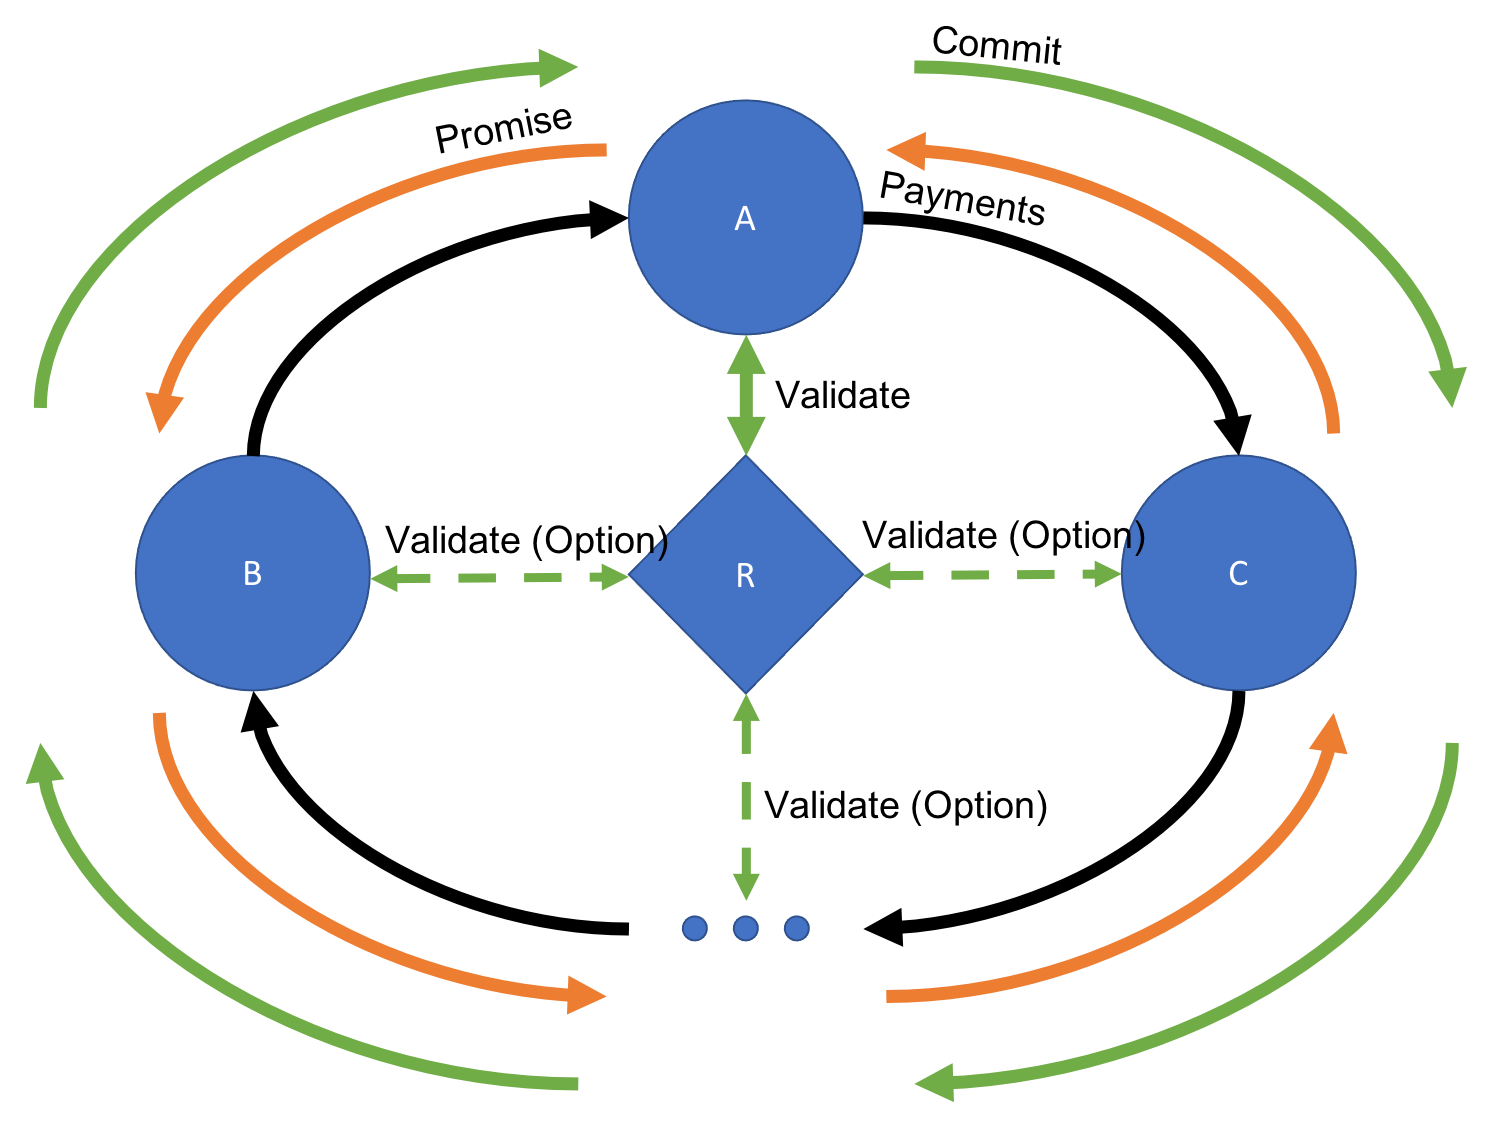
\includegraphics[scale=0.7]{MyCHIPsLiftGraphic.png}
    \caption{Lift Protocol Communication Map}
    \label{fig:liftProt}
\end{figure}

I'll refer to Figure \ref{fig:liftProt} to describe the promise and commit phases of the protocol. In the figure we have 3 nodes that would like to participate in a lift, A, B and C. Node R will serve as the referee for the lift.
The Referee is a well-trusted node in the network that we assume to be honest and have consistent, good communication with all nodes on the network. The Referee will ensure consensus in the case of communication failures.
The ellipsis on the bottom of the circuit represents that a lift could have any number of nodes in the circuit. In the figure, A is the originator of the lift.
Normally the nodes in the lift make payments in the direction of the black arrows. This means that in general, B will have sent A CHIPs, i.e, B owes A some value. During the promise phase messages are sent in the opposite direction (the direction the orange arrows point) and Nodes promise to send CHIPs back to a node who usually pays them. During the commit phase the lift is committed in the same direction CHIPs usually flow in the direction of the Green arrows.

As the originator, Node A will initiate the lift by promising to send CHIPs to Node B conditional upon Node B obtaining and providing the referee's signature to Node A. It does this by creating a lift record that has the lift value, the a network ID of the referee that Node A selects, and a timeout timestamp.
The timeout timestamp will be used to allow a lift that is hanging for a long time to be invalidated.
Although Node A and Node B do not have synchronized clocks, this timeout gives them both a rough idea of how long they may have to wait for the lift to resolve.
The referee's clock is considered authoritative, and the referee will not sign a lift if its clock shows that the timeout has passed. Node A sends this lift record to Node B and promises to send CHIPs if the lift completes.

When Node B or any other node in the cycle receives the lift record, it first confirms that it trusts the referee to be fair and available, and it confirms that the timeout timestamp is acceptable. If the referee is not trusted, or the known route to the target is no longer valid (for instance if it was used in a different lift and the node no longer has debt on that route to clear) it may chose to not continue. The node can optionally return a message indicating that it does not intend to complete the lift, or the node can simply ignore the message. In our model nodes ignore messages if they do not intend to participate in a lift. If a node that receives the lift record wishes to participate it forwards the lift record along with its own promise to the next node in the circuit. 

This continues until the lift record gets returned to the originator (Node A). Then the lift moves into the commit phase and the originator sends the lift record to the referee to request a signature to commit. 

When a referee receives a lift record, it makes sure the that according to it's own clock that the timeout has not been reached. If the Referee decides the lift is not valid it does not provide the signature. Otherwise the referee signs the lift record and returns it's signature to the originator. In either case it records it's result in case a node requests the status of the lift.

When the originator (Node A) receives the signature, it sends it to previous node in the circuit (Node C).  Whenever a node in the circuit receives the the signature, immediately the CHIPs it promised to it's successor are valid. I.e. it has forgiven the debt of it's successor. 
To recover this value it sends the signature it's predecessor. This continues around the circuit until the originator (Node A) receives the signature from its successor (Node B). At this point all nodes have received exactly the amount of chips that they have given and the lift is complete.

At any point, a node can send the lift record to the referee to check the status of a lift. The referee will check with its records to determine if it has made a decision for that lift. If it does have a record it transmits the result including its signature if applicable. If it does not have a result for the lift record yet it checks to see if the lift has timed out or is otherwise invalid. If the lift is invalid, the referee sends a message stating the reason the lift is invalid. Otherwise it returns no signature with a message indicating that the lift is still pending. If, for instance, a node in the circuit failed to continue the lift, in either the promise or the commit phase, the lift would timeout. We don't expect the clocks of individual nodes to be synchronized, but their local clocks should be close enough to know when it is appropriate to ask the referee if a timeout has occurred. By contacting the referee, the nodes that have already promised chips can get a confirmation that the lift is invalidated and they will not need to make good on that promise.
%note a information attack is avoided here where you could send false lifts with different lift ideas to probe the status of transactions.


%Note for Kyle, message from Originator to Termination pre-lift unclear.
%Ask about value fragmentation. I.e. Sure there exists a path of value transfer but the value the entity gives is branched out to many other entities such that no one entity has enough value to make the transfer meaningful. Example: I work for a company and I obtain 100 chips for my labor. That company has 100 customers that each would like to obtain 1 chip's worth of goods. Each of those customers also have similar situations where the value of their work is split among 100 customers. Say a cycle can be found in just 6 steps. Myself, my company, a customer, their company, a customer, merchant I would like to buy from. I would need to execute 10000 separate lifts of 0.01 chips each in order to lift the entirety of my 100 chips. If I would like to spend my money with two merchants this likely would mean I would have to execute 20000 lifts.
\section{Preliminary Results}
The original MyCHIPs lift protocol did not include a referee. Some initial analysis showed that property 1 above was sometimes violated if nodes in the cycle failed to continue a lift. Some nodes were left perpetually waiting for a lift to resolve. To remedy this the timeout feature was added, but this let to a consensus problem and property 3 would sometimes be violated. Fischer, Lynch, and Peterson \cite{Fischer} proved that it is impossible to create a consensus algorithm that is tolerant to even one faulty process. To get around this we introduce the idea of a referee. By assuming that the referee cannot fail and will never lose communication with the network (a very strong assumption), we can guarantee consensus. 

To prove this I modeled a simple 4 node lift in TLA+. First with no referee and noted that property 3 was violated. Then I added the referee and exhaustively proved that the properties hold for a simple 4 node network. To continue this work, we would like to verify that these properties hold for any number of nodes and with any topology. 

\section{Plan of Work}
Model checking the lift protocol quickly becomes intractable as the number of nodes grows large. And model checking cannot provide proof that the protocol works for an arbitrarily large number of nodes. Proving this requires inductive reasoning. I believe that this is provable constructively and I intend to create a mechanical proof in the popular proof assistant Coq. 

A direct approach would be to define a chain of nodes each with their own individual states, and define a set of actions that can be performed that affect those states. Then consider all the actions that are allowable in the protocol to get an implication: if the actions follow the protocol, then these properties hold on the states. This would form a base case for our inductive proof. Then we must prove that if these properties hold for a fixed number of nodes, those properties will still hold with an additional node. This approach is quite difficult. There are many cases to consider and it would take significant automation effort to examine and prove them all. My initial attempts with this approach have been unfruitful.

Instead of taking the direct approach, my strategy for this proof is to utilize an abstraction I call the "sliding window abstraction" to generate an over approximation of the behavior of the system, then use automaton theory to trim out the behaviors that do not follow protocol.

The sliding window abstraction is based on dividing the nodes participating in a lift into equivalence classes based on the phase of the lift they are currently in and--connected with the phase--the actions they can take. For instance, before the lift begins all nodes are in the same equivalence class. Each of them has just one action they can take: initiate a lift. Once a node chooses to initiate a lift we assume it generates and sends it's promise and the lift record to it's successor in one atomic step. The successor now has a new possible action: receive the message. Now there are 3 equivalence classes. The originator is in it's own equivalence class, the successor node is in it's own equivalence class, and all the other nodes remain in their original equivalence class. As the lift progresses along the second node in the chain joins the same equivalence class as the first node. The original equivalence class loses member after member until eventually the last node sends the lift record back to the originator. At that point the originator has a new valid action so it joins a new equivalence class. 

We can observe with this example that as the lift protocol progresses through it's phases there is always a node that is about to transition from one equivalence class to the next. The sliding window abstraction looks only at this node. As this window slides from node to node there are local state variables that change, as well as different actions that the transitioning node could take. We also notice and there are different messages the transitioning node could receive based on the equivalence classes of the nodes directly adjacent to the transitioning node, and the referee. Lets call all these different factors the "window state". We can also observe that many nodes in the cycle will have identical window states.  We can also imagine that if unusual events occur during the lift such as a node faulting for a short time, that this could create unusual combinations of equivalence classes of the adjacent nodes and referee.

Rather then generating these window states by creating a cycle and simulating the sliding the window as the lift progresses, instead we will just consider and evaluate all possible combinations of local state, and equivalence classes of adjacent nodes.  The figure below illustrates this. We need only consider all possible states of the transitioning node T, with every combination of equivalence classes for it's adjacent nodes A, B, and, R. This will over approximate the possible combinations of topology, number of nodes, and failures of nodes.

\begin{figure}
    \centering
    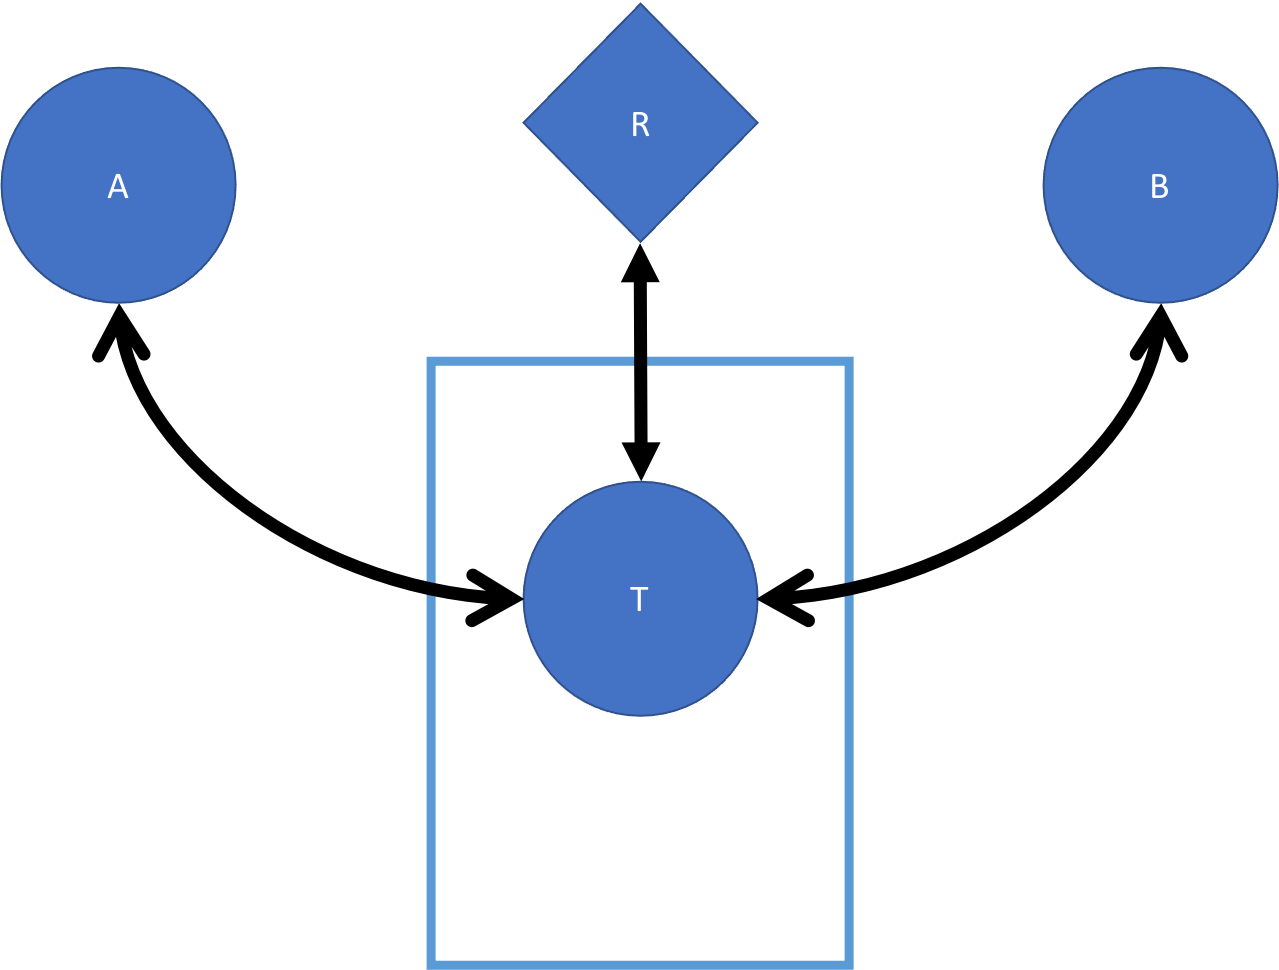
\includegraphics[scale=0.7]{SlidingWindowAbstraction.png}
    \caption{Sliding Window Abstraction}
    \label{fig:slidingWindow}
\end{figure}

For the safety properties, we can consider each window state and determine if the property has been violated. Liveness properties will require further analysis that would involve proving that one window state cannot be reached from another. This should be possible using automaton theory using the actions available in the window state as transitions to determine the next window state.

The protocol makes a distinction between three roles nodes can take: The originator, the referee, and the participant. These roles determine the types of actions a node can take and therefore define distinct equivalence classes to consider as well as the transitions from one equivalence class to another. These are the equivalence classes we have identified:
\begin{enumerate}
\item \textbf{Originator-Pre-Lift --} Actions: Initialize and send lift record, Do nothing
\item \textbf{Originator-Promise-Complete --} Actions: Ask Referee for Signature, Do nothing
\item \textbf{Originator-Commit --} Actions: Send failed message to predecessor, Send Signature to Predecessor, Do nothing

\item \textbf{Referee-Standby --} Actions: Send pending message, Send invalidated message, Do nothing
\item \textbf{Referee-Invalidated --} Actions: Send invalidated message, Do nothing
\item \textbf{Referee-Committed --} Actions: Send signature, Do nothing


\item \textbf{Promise-Pend --} Actions: Ask Referee Status, Do nothing
\item \textbf{Promise-Active --} Actions: Ignore Message, Forward lift record, Ask Referee Status, Fail
\item \textbf{Promise-Pend --} Actions: Ask Referee Status, Fail
\item \textbf{Commit-Active --} Actions: Send signature to predecessor, Do nothing
\item \textbf{Complete --} Actions: Do nothing,

\end{enumerate}

\section{Related Work}
 Bhargavan et. al. Verify Smart Contracts \cite{SmartContracts}. Smart contracts are a type of distributed computation where the program that is executed is secured in a block-chain. While not directly related, smart contracts have the same financial stakes MyCHIPs have and some of their techniques could give inspiration.  Bhargavan et. al, translated the smart contract code into a function programming language, F*, aimed at verification. This allowed for contract verification based on F* type-checking.
 
 
 Fischer, Lynch, and Paterson,\cite{Fischer} prove the impossibility of consensus on even a Boolean, with even one faulty (or malicous) process. However this is only true if the processes don't have synchronized clocks. This proof shows the necessity of the referee with strong reachability requirements for the lift algorithm to always eventually reach consensus on if the lift should commit or be invalidated.
 
 
 Schneider, summarizes and frames many fault tolerant distributed algorithms in the framework of state machines\cite{StateMachine}. He shows how many common algorithms are isomorphic to and can be derived using the state machine approach. It is a helpful method to characterize and compare different approaches.
 
 Lamport\cite{Lamport}, describes a refinement process that takes a distributed fault tolerant consensus algorithm and hardens it to be tolerant of byzantine actors through a process he calls "byzantizing." This method may be useful to ensure the MyCHIPs protocol follows key principles of Byzantine hard protocols.
 
 Delzanno, Tatarek, and Traverso, model check a common consensus algorithm called Paxos in Spin. Their spin constructs provide helpful examples of how distributed algorithms are efficiently modeled.\cite{Delzanno_2014}
 
 Konnov, Veith, and Widder explore the unsolved problems associated with model checking distributed algorithms. This can serve as a hazard map of difficult unsolved problems. It would be unfortunate if solving a known problem that is tangential to my work becomes prerequisite to finishing. This also can serve to give context to how my work and show how it progresses towards solving some of these problems.\cite{Konnov}

\bibliographystyle{unsrt}
\bibliography{proposal}

\end{document}
